\author{Марухленко Д.С. @japersik}
\date{\today}

\documentclass[a4paper,12pt]{article}
\usepackage[english,russian]{babel}
\usepackage[utf8]{inputenc}
\usepackage{amsmath,amsfonts,amssymb,amsthm,mathtools}
\usepackage{hyperref}
\usepackage{wrapfig}

\usepackage[left=2.5cm, right=1.5cm, top=2.5cm, bottom=2.5cm]{geometry}
\usepackage{array}
\usepackage{tabularx}
\usepackage{indentfirst}
\usepackage{stmaryrd}
\usepackage{graphicx}
\setlength\parindent{5ex}

\usepackage{fancyhdr} %%колонтикулы
\usepackage{lastpage}
\pagestyle{fancy}
\fancyhf{}
\rfoot{\thepage}
\cfoot{}
\lfoot{}
\renewcommand{\footrulewidth}{0.4pt}

\usepackage{lipsum}
\usepackage{wasysym}
\usepackage{booktabs}
\usepackage{blindtext}
\usepackage{siunitx}


\usepackage{svg}

\newcommand{\authorName}{Марухленко Д.С}
\newcommand{\workType}{Задача №1}
\newcommand{\workName}{Математическое моделирование двухмассового механизма}
\newcommand{\subjectName}{Системы управления в электроприводе}
\newcommand{\workOption}{Вариант №14}
\newcommand{\groupNumber}{R34352}
\newcommand{\teacherName}{Демидова Г.Л.}

\begin{document}
    \thispagestyle{empty}
%титульный лист%
\begin{center}
    Национальный исследовательский университет ИТМО\\
    Факультет систем управления и робототехники
    \vskip 7cm

    \Huge \workType                         \\
    \huge <<\workName>>                     \\
    \Large по дисциплине <<\subjectName>>   \\
    \large \workOption
\end{center}
\vfill

\begin{flushright}
    Подготовили: \authorName         \\
    Группа: \groupNumber            \\
    Преподаватель: \teacherName     \\
\end{flushright}
\vskip 2cm

\begin{center}
    Санкт-Петербург 2022г.
\end{center}
\newpage
    \section{Цель работы}
\begin{enumerate}
    \item Рассчитать коэффициент датчика момента из условия поддержания номинального
    момента при величине напряжения задания 10В.
    \item Параметры ПИ-регулятора момента из условия настройки системы на
    технический оптимум.
    \item Реализовать математическую модель контура в пакете MATLAB.
    \item Снять реакции $M(t)$, $U_y(t)$, $\varepsilon(t)$ на скачкообразное изменение задающего воздействия
    при нулевых начальных условиях, исключив влияние эл. /мех. связи. Определить
    параметры $M(t)$: время первого согласования $t_\text{p1}$, перерегулирование, время переходного
    процесса $t_\text{п}$ и сравнить с параметрами эталонной кривой.
    \item Выполнить программу п.4 c учетом эл./мех. связи.
\end{enumerate}



\section{Данные варианта}
\begin{itemize}
    \item Nпп: 14
    \item $\omega_\text{0ном}$: 706 (1/c)
    \item $M_\text{ном}$: 13.7 (Нм)
    \item $M_\text{п}$: 24.7 (Нм)
    \item $J_\text{1}$: 0.008 (кгм$^2$)
    \item $J_\text{2}$: 0.0025 (кгм$^2$)
    \item $C_\text{12}$: 300
    \item $T_\text{э}$: 50 (мс)
    \item $T_\text{пр}$: 10 (мс)
    \item $K_\text{пр}$: 15
    \item $M_\text{с1}$: 10 (Нм)
    \item $M_\text{с2}$: 3.7 (Нм)
\end{itemize}
\newpage
    \section{Марериалы работы}
\subsection{Расчет переходных процессов}
Так как нам известна электромагнитная постоянная, рассчитаем электромеханическую постоянную и статическую жесткость.
\begin{gather*}
    \beta = \frac{M_\text{п}}{\omega_\text{ном}}=0.035\\
    T_M = \frac{J_1+J_2}{\beta} = 0.3001
\end{gather*}
Из отношения $4T_\text{э}<T_\text{М}$ имеем два вещественных корня передаточной функции.
Составим характеристическое уравнение и найдем его корни:
\begin{gather*}
    T_\text{э}T_\text{М}\lambda^2+ T_\text{М}\lambda + 1 = 0\\
    \lambda_1 =   -4.2242\\
    \lambda_2 =    -15.7758
\end{gather*}
Определим время переходного процесса:
\begin{gather*}
    t_\text{п} = \frac{3}{|\lambda_1|} = 0.7102
\end{gather*}
\newpage
\subsection{Одномассовый механизм}
Запишем математическую модель ДПТ с одномассовым механизмом в виде системы дифференциальных уравнений

\begin{gather*}
    \begin{cases}
        \dot{M} = \frac{\beta}{T_\text{э}}\omega_0-\frac{1}{T_\text{э}}M-\frac{\beta}{T_\text{э}}\omega_1\\
        \dot{\omega}_1 = \frac{M}{\beta T_M}-\frac{M_c}{\beta T_M}
    \end{cases}
\end{gather*}
Преобразуем уравнения в систему вида вход-состояние-выход в матричной форме
\begin{gather*}
    \begin{bmatrix}
        \dot{M} \\
        \dot{\omega}_1
    \end{bmatrix}
    =
    \begin{bmatrix}
        -\frac{1}{T_\text{э}} & -\frac{\beta}{T_\text{э}}\\
        -\frac{1}{\beta T_\text{M}} & 0
    \end{bmatrix}
    \begin{bmatrix}
        M \\
        \omega_1
    \end{bmatrix}+
    \begin{bmatrix}
        \frac{\beta}{T_\text{э}}&0\\
        0&\frac{1}{\beta T_M}\\
    \end{bmatrix}
    \begin{bmatrix}
        \omega_0\\
        M_c
    \end{bmatrix}
\end{gather*}
Проведем моделирование системы при $\omega_0 = 0$, $M_c = 0.1M_\text{ном}$
\begin{figure}[!h]
    \centering
    \begin{minipage}{0.5\textwidth}
        \centering
        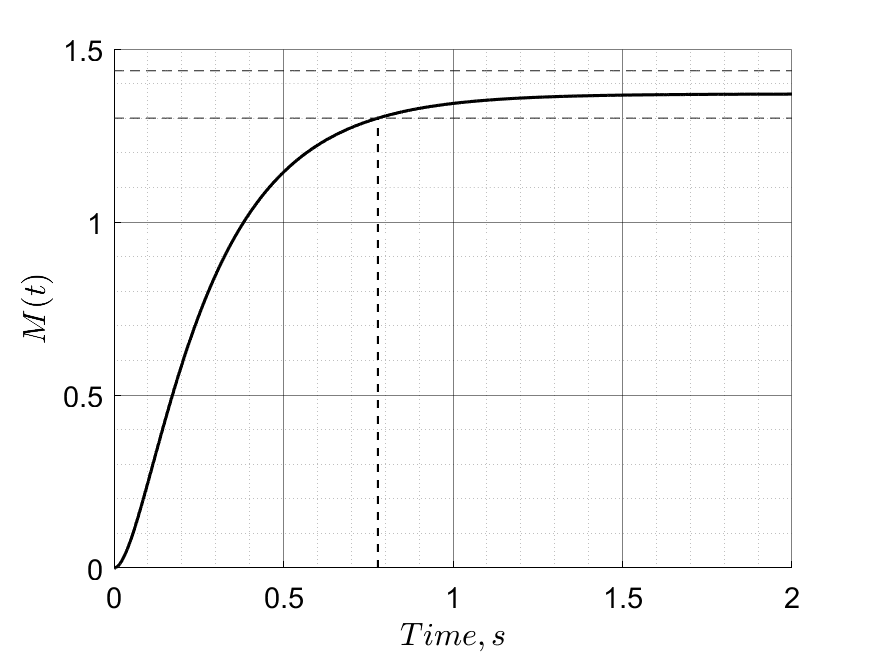
\includegraphics[width = \textwidth]{img/task12_M}
        \label{fig:img/task12_M}
    \end{minipage}%
    \begin{minipage}{0.5\textwidth}
        \centering
        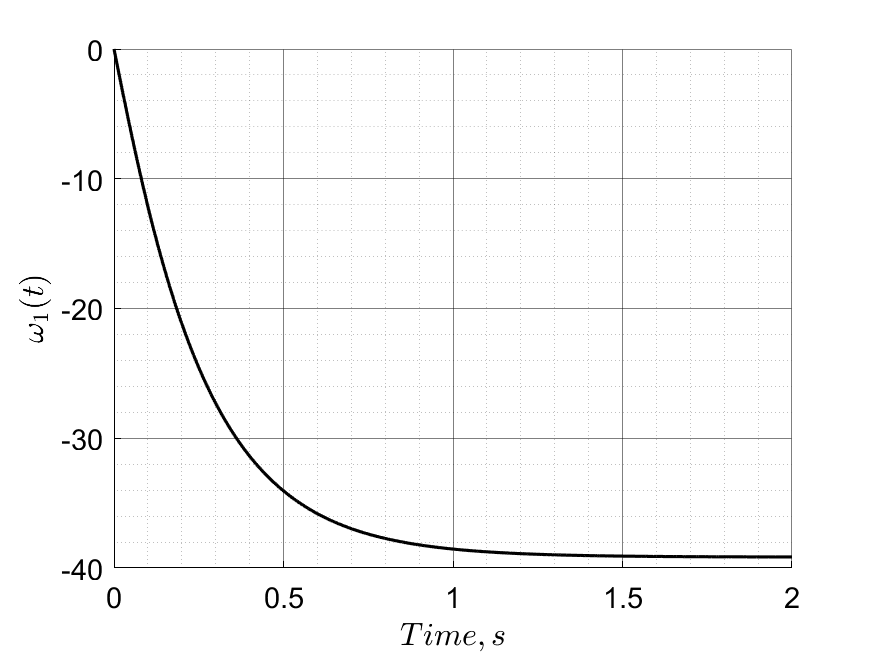
\includegraphics[width = \textwidth]{img/task12_omega1}
        \label{fig:img/task12_omega1}
    \end{minipage}%
    \caption{Результат моделирования системы при $\omega_0 = 0$, $M_c = 0.1M_\text{ном}$}
\end{figure}

Проведем моделирование системы при $\omega_0 = 0.1\omega_\text{ном}$, $M_c = 0$
\begin{figure}[!h]
    \centering
    \begin{minipage}{0.5\textwidth}
        \centering
        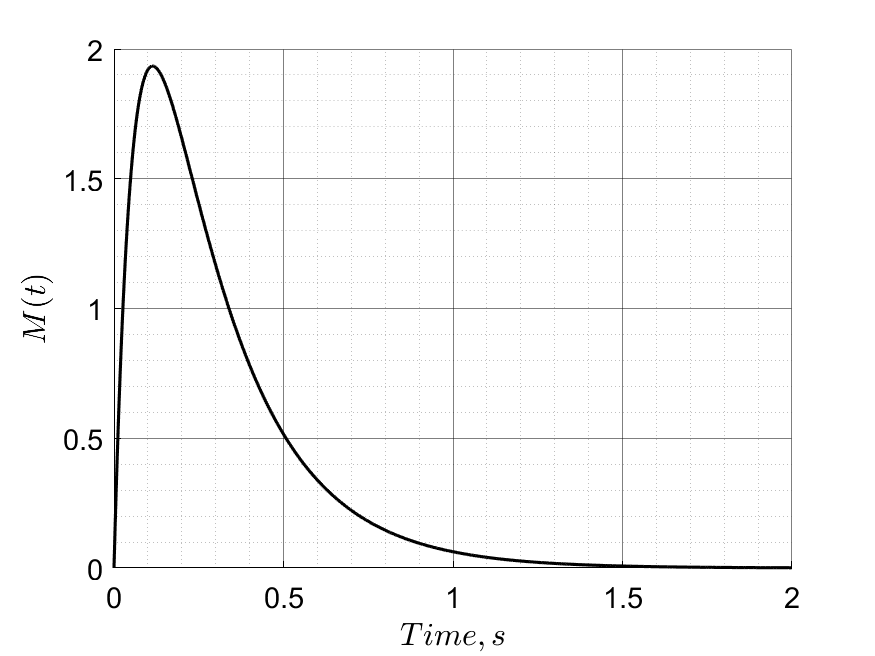
\includegraphics[width = \textwidth]{img/task11_M}
        \label{fig:img/task11_M}
    \end{minipage}%
    \begin{minipage}{0.5\textwidth}
        \centering
        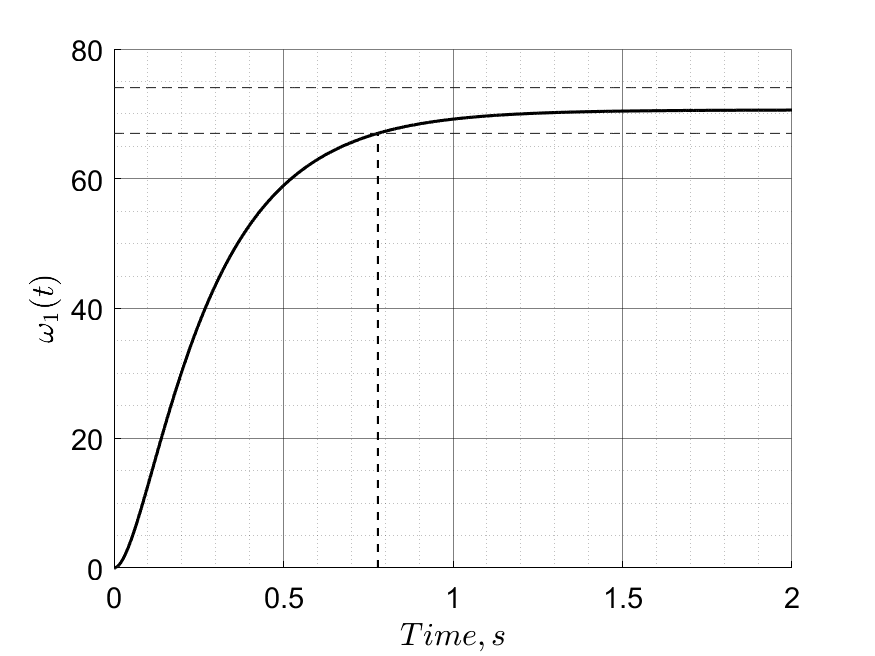
\includegraphics[width = \textwidth]{img/task11_omega1}
        \label{fig:img/task11_omega1}
    \end{minipage}%
    \caption{Результат моделирования системы при $\omega_0 = 0.1\omega_\text{ном}$, $M_c = 0$}
\end{figure}

\subsection{Двухмассовый механизм}
Запишем математическую модель ДПТ с двухмассовым механизмом в виде системы дифференциальных уравнений
\begin{gather*}
    \begin{cases}
        \dot{M} = \frac{\beta}{T_\text{э}}\omega_0-\frac{\beta}{T_\text{э}}M-\frac{\beta}{T_\text{э}}\omega_1\\
        \dot{\omega}_1 = \frac{M}{J_1}-\frac{M_{12}}{J_1}-\frac{M_{c1}}{J_1}\\
        \dot{M}_{12} = C_{12}\omega_1 -C_{12}-\omega_2\\
        \dot{\omega}_2 = \frac{M_2}{J_2}-\frac{M_{c2}}{J_2}
    \end{cases}
\end{gather*}
Преобразуем уравнения в систему вида вход-состояние-выход в матричной форме
\begin{gather*}
    \begin{bmatrix}
        \dot{M} \\
        \dot{\omega}_1\\
        \dot{M}_{12} \\
        \dot{\omega}_2
    \end{bmatrix}
    =
    \begin{bmatrix}
        -\frac{\beta}{T_\text{э}}&-\frac{\beta}{T_\text{э}}&0&0\\
        \frac{1}{J_1} 0 -\frac{1}{J_1} 0 \\
        0&C_{12}&0&-C_{12}\\
        0&0&J_2&0\\
    \end{bmatrix}
    \begin{bmatrix}
        M \\
        \omega_1\\
        M_{12} \\
        \omega_2
    \end{bmatrix}+
    \begin{bmatrix}
        \frac{\beta}{T_\text{э}}&0&0\\
        0 & -\frac{1}{J_1}&0\\
        0&0&0\\
        0&0&\frac{1}{J_2}\\
    \end{bmatrix}
    \begin{bmatrix}
        \omega_0\\
        M_{c1}\\
        M_{c2}\\
    \end{bmatrix}
\end{gather*}

Проведем моделирование системы при $\omega_0 = 0$, $M_c = 0.1M_\text{ном}$
\begin{figure}[!h]
    \centering
    \begin{minipage}{0.5\textwidth}
        \centering
        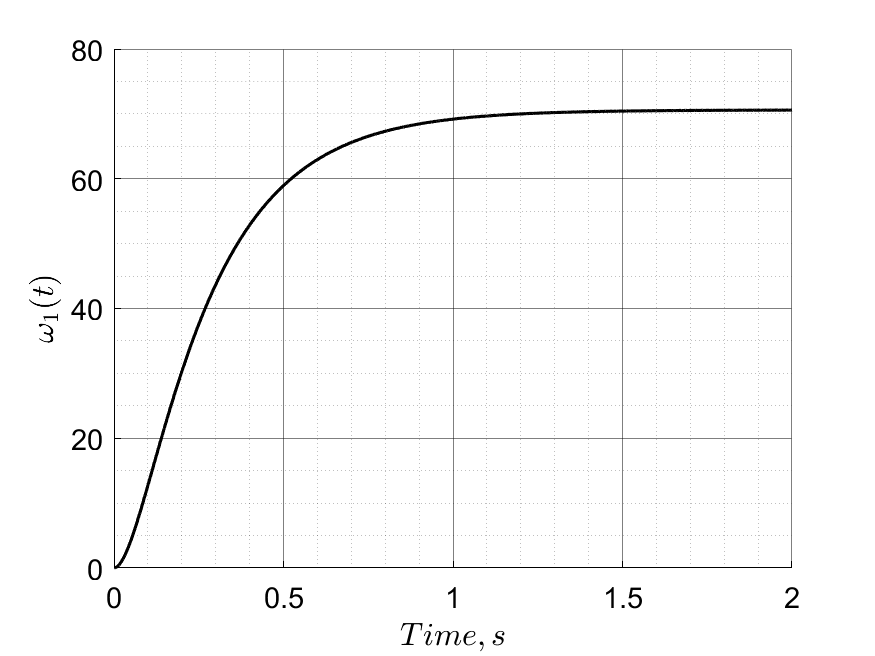
\includegraphics[width = \textwidth]{img/task21_omega1}
        \label{fig:img/task21_omega1}
    \end{minipage}%
    \begin{minipage}{0.5\textwidth}
        \centering
        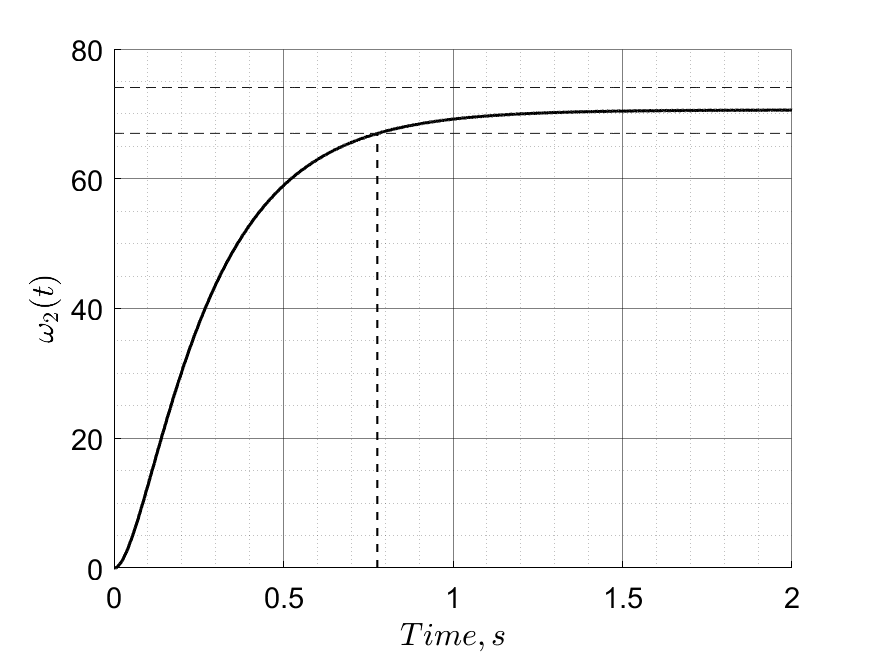
\includegraphics[width = \textwidth]{img/task21_omega2}
        \label{fig:img/task21_omega2}
    \end{minipage}
    \begin{minipage}{0.5\textwidth}
        \centering
        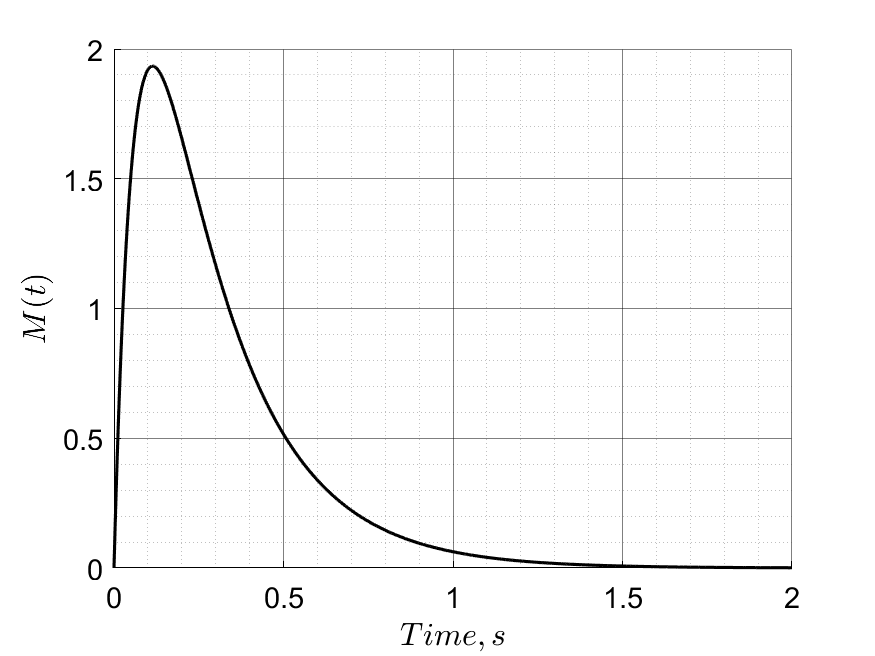
\includegraphics[width = \textwidth]{img/task21_M}
        \label{fig:img/task21_M}
    \end{minipage}%
    \begin{minipage}{0.5\textwidth}
        \centering
        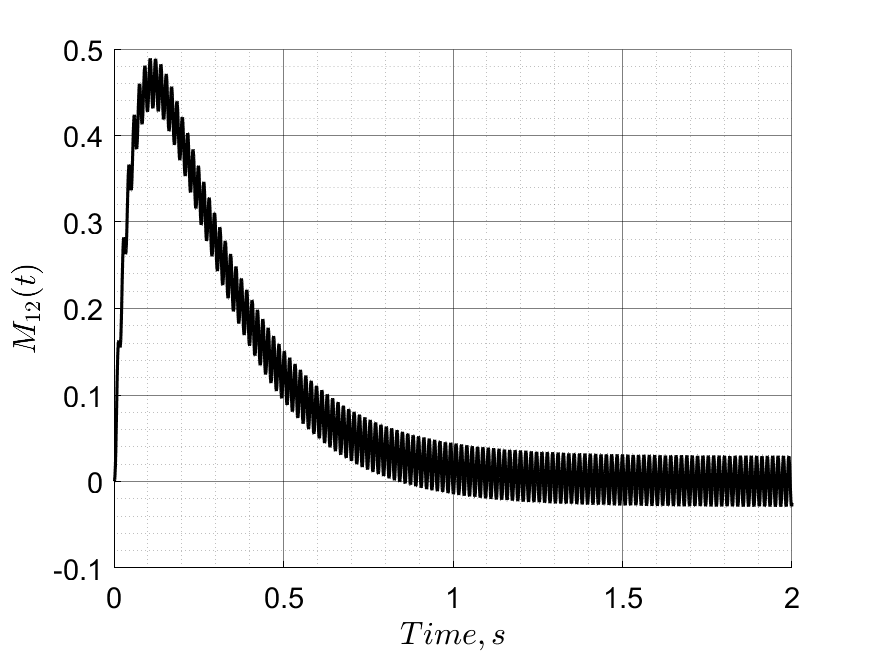
\includegraphics[width = \textwidth]{img/task21_M12}
        \label{fig:img/task21_M12}
    \end{minipage}%
    \caption{Результат моделирования системы при $\omega_0 = 0$, $M_c = 0.1M_\text{ном}$}
\end{figure}

 \newpage
Проведем моделирование системы при $\omega_0 = 0.1\omega_\text{ном}$, $M_c = 0$
\begin{figure}[!h]
    \centering
    \begin{minipage}{0.5\textwidth}
        \centering
        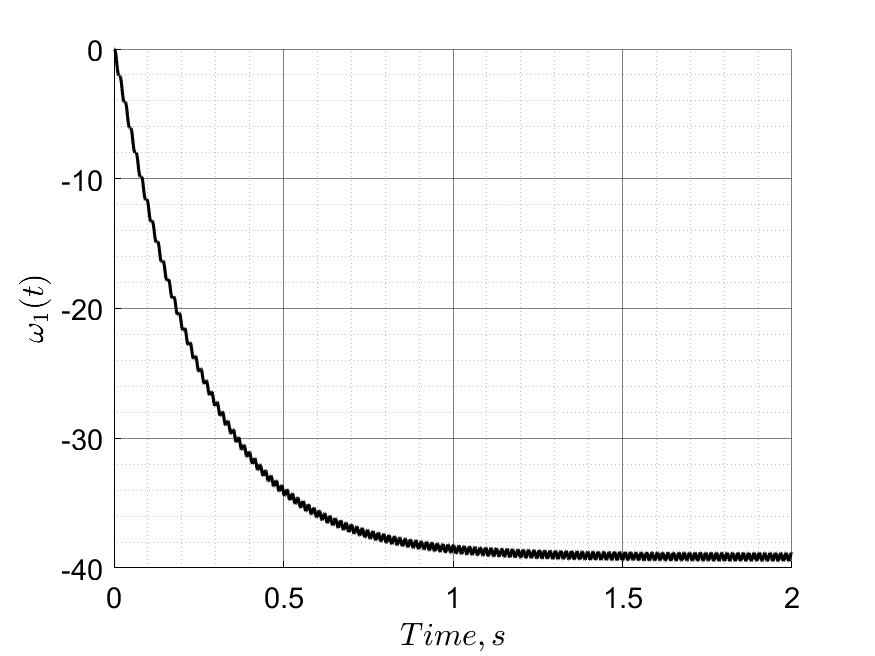
\includegraphics[width = \textwidth]{img/task22_omega1}
        \label{fig:img/task22_omega1}
    \end{minipage}%
    \begin{minipage}{0.5\textwidth}
        \centering
        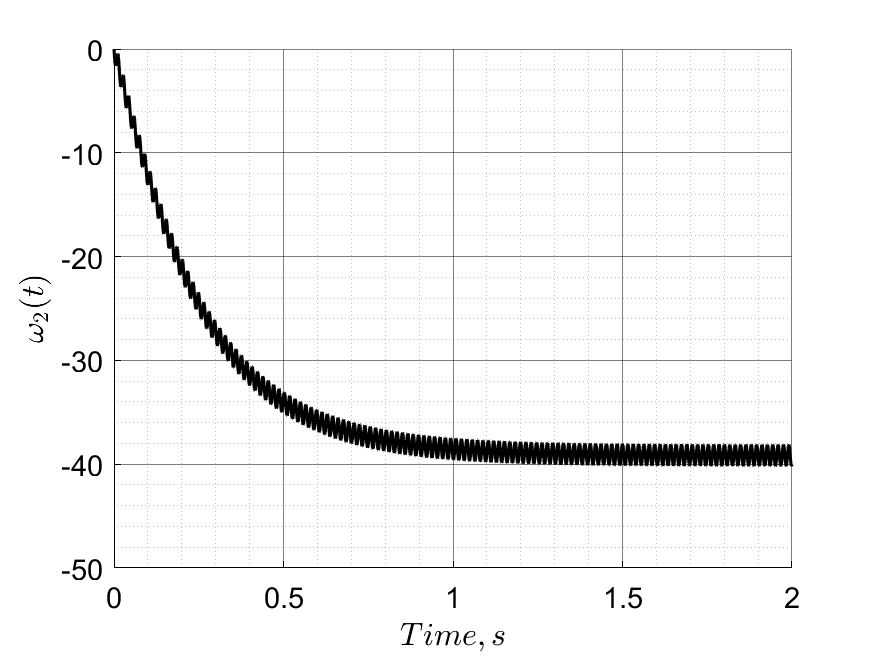
\includegraphics[width = \textwidth]{img/task22_omega2}
        \label{fig:img/task22_omega2}
    \end{minipage}
    \begin{minipage}{0.5\textwidth}
        \centering
        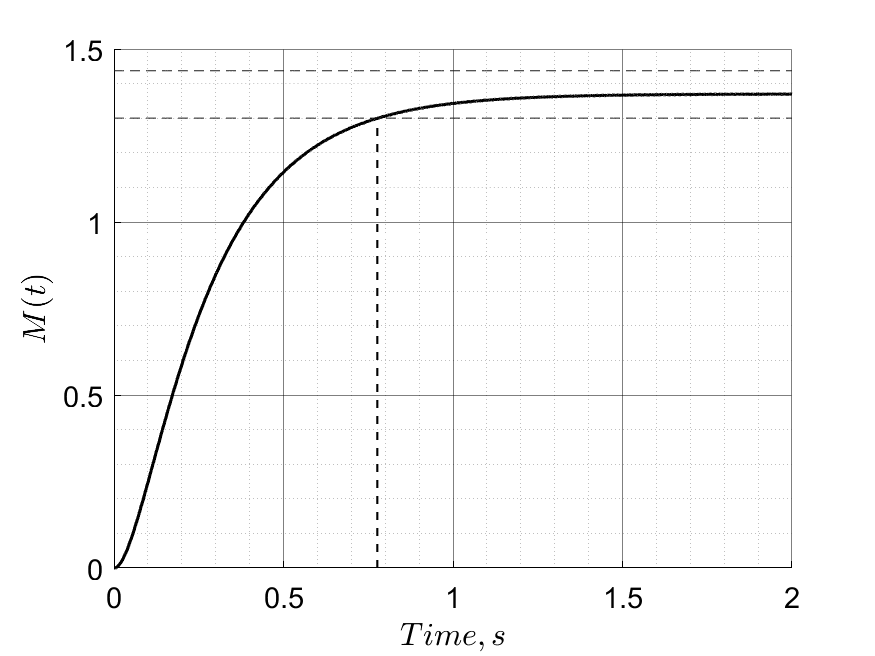
\includegraphics[width = \textwidth]{img/task22_M}
        \label{fig:img/task22_M}
    \end{minipage}%
    \begin{minipage}{0.5\textwidth}
        \centering
        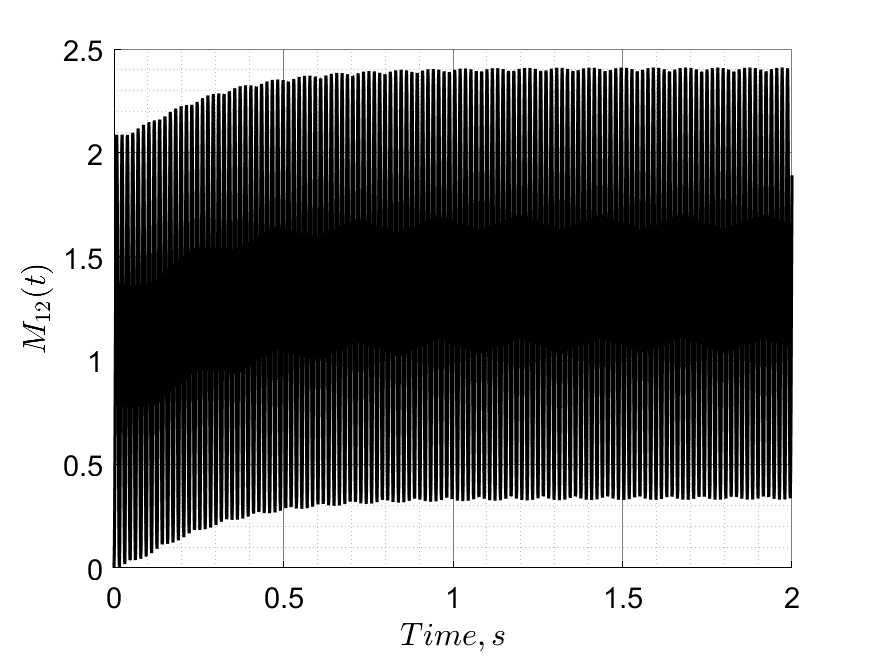
\includegraphics[width = \textwidth]{img/task22_M12}
        \label{fig:img/task22_M12}
    \end{minipage}%
    \caption{Результат моделирования системы при $\omega_0 = 0$, $M_c = 0.1M_\text{ном}$}
\end{figure}

    \section{Вывод}

В ходе работы был синтезирован унифицированный контур регулирования момента.
Результат моделирования показал, что моделирование без электромеханической связи установившаяся ошибка регулирования пренебрежительно мала и, возможно, связано с неточностями компьютерных вычислений чисел с плавающей точкой.
При моделировании с учетом влияния электромеханических связей существует малая установившаяся ошибка, которая же вызывает неограниченный рост управления.
\end{document}